\chapter{Lezione 2 - Enterprise resource planning}

Benvenuti a tutti a questa lezione sull'enterprise resource planning, gestione delle risorse di un'impresa, di un'azienda o di un'organizzazione.
Quali sono gli argomenti che affronteremo in questa lezione?

Argomenti trattati:

\FloatBarrier
\begin{figure}[H]
  \centering
  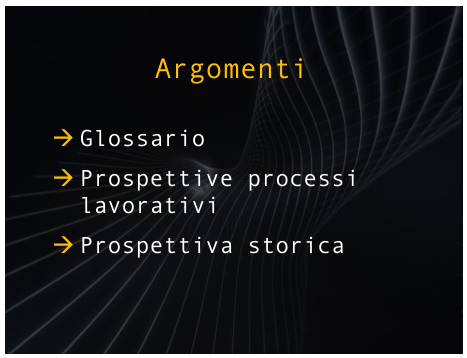
\includegraphics[width=0.50\textwidth,
                    trim=40 80 40 40, % L B R T
                    clip]
                    {images/Lez02_p01_fig_02}
  \caption{Sommario}
  \label{fig:Lez15_p06_fig_02}
\end{figure}
\FloatBarrier
\noindent

Innanzitutto faremo il punto sulla terminologia, quindi vedremo alcune definizioni dei termini, confronteremo alcuni termini più complessi delle locuzioni riguardanti questo settore.
In seguito vedremo quali sono le prospettive da cui vengono analizzati i processi aziendali, sono due prospettive che vedremo.
Da ultimo il terzo argomento che vedremo in questa parte della lezione, faremo una prospettiva storica dei sistemi che sostengono, aiutano nella gestione e nella pianificazione delle risorse aziendali.

\section{Glossario}

